%\nonstopmode
\hbadness=100000
\documentclass[a4paper, 12pt]{article}
\usepackage{verbatim,amsmath,graphicx,geometry,textcomp,url,caption,float,titlesec,setspace,paralist}
\geometry{ a4paper, total={186mm,273mm}, left=12mm, top=8mm}
%setting spacing
\titlespacing{\section}{0pt}{0.1cm}{0cm}
\titlespacing{\subsection}{0pt}{0.1cm}{0cm}
\titlespacing{\subsubsection}{0pt}{0.1cm}{0cm}
\titlespacing{\paragraph}{0pt}{0.1cm}{0cm}
\setlength{\itemsep}{0cm}

\usepackage[toc, page]{appendix}
\usepackage[dvipsnames]{xcolor}
\definecolor{subr}{rgb}{0.8, 0.33, 0.0}
\definecolor{func}{rgb}{0.76, 0.6, 0.42}
\begin{document}
\begin{center}
MCNP Report										\\
Ocean Wong (Hoi Yeung Wong)						\\
MSc Physics and Technology of Nuclear Reactors	\\
2019-03-09 										\\
\textbf{Abstract}
Abstract yet to be written
\end{center}

\section{Introduction}
See the Appendices for the geometries and materials definitions of the following problems.
\subsection{Exercise 1: Simple Neutron Source in a Bucket of Water}
A narrow, stainless steel water bath is subjected to a point source of (uranium thermal fission) neutron near it's bottom. The neutron fluences and spectra measured just outside each of the faces of the neutron bath are examined. 
\subsection{Exercise 3: Criticality}
A square water bath with four short, fully-submerged enriched Uranium cylinders, arranged in a ``plus" sign, is shown to be supercritical when moderated by pure water, even when it is only enriched to e=20\%. The aim of the exercise is to find the minimum degree of boronation in the water required to keep the system subcritical to $\text{k}_{\text{eff}}<0.8$ when the cylinders are enriched to e=25\%.

\section{Method}
\subsection{Technicalities for reproducibility}
\paragraph{Software and hardware specifications\indent} For the following exercise all cross-section data were retrieved from the ENDL92 library (the most recently updated library available, acquired by Lawrence Livermore National Laboratory) and simulated in MCNP 4C2, ran on the phymat server of University of Birmingham School of Physics and Astronomy, which is a Scientific Linux 7.3 (Nitrogen) system with 16 CPU's (Intel(R) Xeon(R) CPU E5-2630 v3 @ 2.40GHz) (though only 1 CPU is used at a time).
\paragraph{Reproducibility of the .ip files} In both cases, the default random number control 0.727343232450560E+14 was used, and the centre of the stainless steel tank's exterior surfaces was placed at the origin.
\paragraph{Material definition} The isotopic composition of water was retrieved from [4]; the elemental composition of other materials were provided by the problem sheet, and were all assumed to have the same isotopic compositions as naturally occuring elements stored by the default AAA=000 option in the ZAIDs identifier. See the tables in the Appendix for more.
\paragraph{Geometry definitions\indent} The geometry for exercise 1 and 3 were set to the dimensions as required by the problem sheet; the cross-sections of their geometries are shown in Figure \ref{Ex1CrxSx} and \ref{Ex3CrxSx} in the Appendices.
\paragraph{Energy cutoff\indent}
Energy cutoff is not applied so that very slow (thermalized) neutrons are allowed to interact and let further reactions take place.

\subsection{Exercise 1}
\paragraph{Tallies\indent}
Therefore for exercise 1, the lower bound of the $1^{st}$ bin of each tally is E=0.

The temperature of the cross-section data in databse 42(ENDL92) were acrquired at T=300K, as shown in 91-99, and is subsequently adjusted down to 20.4 ${}^{o}$C ($2.53 \times 10^{-8}$MeV) when running the simulation. Either way, thermal effects should significantly affect that falls into the first 3 energy bins. ($0$-$10^{-9}$MeV, $10^{-9}$-$10^{-8}$MeV,$10^{-8}$-$10^{-7}$MeV respectively).

The tally probability distributions (histograms shown in table 161) all show reasonably Gaussian distributions (and the cumulative probability distributions all show reasonably sigmoidal distributions) without the majority of the counts falling into a single bin; therefore there is no inherent need for using a finer spacing; but for the purpose of visualizing the spectrum with a higher resolution, a finer group structure with trifolded bin density (still logarithmically spaced, 3 bins per decade) was used.

Even when the spacing of energy groups is trisected in this manner, the $1^{st}$ bin ($0$ to $1\times 10^{-9}$ MeV) is still the bin that receives the least counts. In a real problem this would have been merged with the $2^{nd}$ bin to form a single, larger bin to tally up all the completely thermalized neutrons, increasing its count so that it converges to a precise enough value in a shorter CPU time; but according to the constraint of the problem, there must be one bin with ${10^{-9}}$ MeV as the upper limit. Therefore the only option left is to increase the number of histories such that the results of this bin converges.

\paragraph{Number of particles}
Due to the large cross section in the thermal region which increases as the neutron slows, very few neutrons of these energies can travel far enough to be counted by these surface flux tallies. Therefore this bin always have the largest relative errors among all bins. To ensure that no bins have relative error larger than 0.10 such that the results are reliable, enough histories must be ran to allow the $1^{st}$ energy bins in all 3 tallies to be filled sufficiently, in addition to passing all 10 statistical checks.

The number of particles required is discussed in detail in section \ref{Ex1NumHist}.

\paragraph{Source location\indent}By examining the first 50 particles(using \texttt{PRINT 110}), the source was confirmed to be a point souce 2cm above the centre of the bottom of the tank's internal surface; and the majority of the particles have initial energy $E<4$ MeV as expected when they are distributed according to the Watt spectrum for neutron generated by ${}^{235}U$+n(thermal) (See the Watt spectrum in Figure \ref{Watt}).

\subsection{Exercise 3}
\paragraph{Note on cross-section library\indent} There is no delayed neutron cross section data available in ENDL92 (or any other nuclear databases available on phymat), so the simulation may deviate from reality slightly. There is no workaround for this issue; but one can assume, for the purpose of this simulation, that a cross-section database without delayed neutron cross-section should be accurate enough.

\paragraph{Geometry definition\indent} It is easier to define the geometry if a sphere was used to define the graveyard (void) outside (where neutron importance=0); but a cuboidal geometry was chosen instead to allow the surface flux detectors (F2) to tally particles passing through lateral surfaces separately from particles passing through horizontal surfaces.

All components except the concrete floor had the same neutron importance. Neutron importance in concrete started off at 1 but was subsequently reduced to 0.1 such that the simulation runs faster by ignoring particles that enter the concrete, since they will otherwise undergo a lot of collision (each requiring a lot of CPU time) to slow down, without causing multiplication.

If the mean free path to absorption $\lambda_{\text{abs}}$ is known, the dimension of the concrete floor can be chosen to extend from the stainless steel tank by $N\lambda_{\text{abs}}$ where N is some arbitrary threshold factor (e.g. 3).
However only the mean free path to collision for neutron is found on a cell particle activity table (using \texttt{PRINT 126}). Since concrete is only a weakly neutron-absorbing medium, this \emph{cannot} be used as the proxy for $\lambda_{\text{abs}}$. 
Instead the fraction of neutrons escaping the concrete block into the void was measured. This was done by comparing the number of neutrons travelling from the concrete to the void region (where neutron importance = 0) (measured with a surface flux tally card) to the neutron population in the concrete. The quantity ``population" instead of ``tracks entering" was used because the latter re-counts particles re-entering the same cell, thus the former is a more accurate measurement of how many distinct neutrons have been present in the concrete block. The simulation is considered accurate when the ratio of these two numbers is less than 1\%, i.e. $<$ 1\% of the neutrons entering the concrete were ``killed" (by entering the void region) instead of being absorbed in the concrete/reflected back towards the tank. The dimension of the concrete block was increased until this ratio is lower than 1\%.

This resulted in a concrete floor block of 160.4cm in the x- and y-directions and 50 cm in the z-direction, resulting in 0.21621209\%  and 0.04494092\% of neutrons escaping through the lateral planes and the horizontal plane (plane separating the concrete block from the void below) respectively. This was used as the final dimension for the concrete block.

\paragraph{Source definition\indent}
Using the \texttt{KSRC} card a ``generic Watt spectrum"[1] of neutrons were created at the center points of each cylinder.
\\This allowed for very fast convergence of the results, where the $\text{k}_{\text{eff}}$ value settled down to a stable value in less than 10 generations. The $\text{k}_{\text{eff}}$ estimation started after that.

The alternatives of using an \texttt{SDEF} card with a cookie cutter(\texttt{CCC}) rejection/\texttt{CEL} rejection OR 5 uniform cylindrical sources overlayed onto cell 11-15 (all the uranium cylinder cells) were attempted, but were not applied in the end because it is likely to distribute neutrons close to the non-re-entrant surfaces where they can escape, reducing the effectiveness of the source and potentially increasing the number of cycles that needs to be skipped. [2]

\paragraph{Choices of number of particles and number of cycles\indent}
3000 particles per cycle were shown to give a $\text{k}_{\text{eff}}$ that converges in $\approx$10 cycles; 5000 particles per cycles were shown to give faster convergence of $\text{k}_{\text{eff}}$ value (in $<$ 5 cycles), but further increase in number of particles per cycles to 8000 did not show significant improvemence in speed of convergence. Therefore the number of particles were chosen to be 5000, and to be servative, the first 10 cycles were skipped (ikz=10).

At 5000 particles per cycle, $\text{k}_{\text{eff}}$ was shown to converge sufficiently by the 500${}^{th}$ cycle; further increase in total number of cycles yields deminishing marginal increase in precision at the cost of increasing the computing time, asymptotically approaching 0; thus only 500 cycles were ran, requiring 10.27 minutes of computing time.

The number of cycles to run per simulation were later changed when the $\text{k}_{\text{eff}}$ changed. For details see section \ref{Ex3NumHist}.

\paragraph{Alteration to material definition\indent} For ease of changing the input file, when attempting to find a concentration of boron that gives a solution, the excess boron is added \emph{on top of} the existing weight fractions for hydrogen and oxygen, the latter two already summed to unity. This results in a weight fraction of boronated water with larger-than-unity, unnormalized weight fraction; and only this excess weight fraction of boron was changed between iterations, allowing MCNP to calculated the normalized the weight fraction of boron in water before running each simulation. The resulting, correctly normalized weight fraction of boron is printed in table 40.

\section{Result}
\subsection{Exercise 1}
\begin{table}[H]
	\centering
	\begin{tabular}{cccc}
		tally (surface(s)) & 12 (surface (21 22)) & 22 (surface (23 24)) & 32 (surface 25)	\\
		average energy (keV)  &609.969 & 99.755  & 726.59 \\
		average energy (keV)  &626.966 & 104.393 & 731.702
	\end{tabular}
	\caption{Arithmatic mean of the energy of neutrons recorded in the various tallies.
	For comparison the Watt spectrum used reaches maximum emission probability density at 0.769 MeV (Figure \ref{Watt}).
	}\label{Ex1meanE}
\end{table}
[dividing by the difference in upper and lower class boundaries so that it gives number density instead?]
\\*Insert spectrum (histograms) of the 3 tallies
\\*plot variation of mean (using data from all)
\\*plot variation of error(using data from all)
\\*plot variation of VoV (using data from all)
\\*plot variation of fom (using data from all)
\subsection{Exercise 3}
keff variation plot by cycle number and \\* confidence interval

\section{Analysis and discussion}
Note:from the Watt spectrum (Figure \ref{Watt}) that there is a small but non-zero probability of getting neutrons of very high energy. This leads to some warning messages when the occassional particle scores above the upper limit of the largest tallying bin in Exercise 1.

\subsection{Answer to numbered questions for Exercise 1}\label{Ex1Ans}
\begin{compactenum}
	\item These results has limited reliability because the last statistical check (pdf slope=decreasing?) for tally 22 and 32 were not passed, meaning that some reactions are not sampled enough for us to be confidence about the frequencies of their occurance.
	\\Additionally, some bins in the PDF are empty (seen table 161 of tally 22) suggesting that insufficient number of neutrons is sampled to approximate a continuous distribution.
	\item Using the notation $\Phi_i$ = fluence calculated for the i${}^{th}$ energy bin \emph{per history},
	\\N = number of histories = 20,000,
	\begin{table}[H]
		\centering
		\begin{tabular}{cccc}
			tally (surface(s)) & 12 (surface (21 22)) & 22 (surface (23 24)) & 32 (surface 25)	\\
			fluence (cm$^{-2}$) &14.9502  & 4.79592 & 68.4946 \\
			fluence (cm$^{-2}$) &15.36682 & 5.01888 & 68.9764
		\end{tabular}
		\caption{ The total fluences $\Phi$ are simply calculated by formula $N \sum\limits_i (\Phi_i)$ , unit = 1/cm${}^{2}$
		}\label{Ex1Fluences}
	\end{table}
	\item Both the spectra and the mean energy of the tallies reflects that the hardness of neutron spectrum decreases as follows: hardness at base (Tally 32)$>$long side (Tally 12)$>$short side (Tally 22).
	This is because distance of them increases in that order.
	\\*The ratio of neutron flux in the slow/Cadmium region ($<$0.01 MeV) to neutron flux in the resonance regions ($>$0.01MeV) builds up since the latter gets slowed down/captured by the resonance peaks much faster than the rate of consumption of the former, as they travel through the material.
	\\More neutrons can penetrate the base at the energy its creation energy without being moderated by the water; therefore the $1^{st}$ bin of tally 32is more filled than that of tally 12. 
	\\The fluence also decrease in the same order as a result of the inverse square law and the capture of neutron by water when it has to travel through a longer distance in water.
\end{compactenum}
After this I need to compare the 280000 histories with this.(\\*Discuss these results in relation to the three questions posed above?)
\subsubsection{Number of histories required to converge}\label{Ex1NumHist}
Even after running 500,000 histories, the relative error for this $1^{st}$ bin remains high ($0.2599$, $0.4236$, $0.3681$, for tally 12, 22, and 32, respectively) despite the fact that all other statistical checks were passed after running 500,000 histories, and the fom has alreay converged to a reasonably stable asymptotic limit.

If one does not care for the accuracy of the $1^{st}$ bin, then running 2,800,000 histories is sufficient, as it passess all statistical test, and produces a sufficient number of dancing, in a reasonable computing time of 1.98 minutes. However, 18,000,000 histories are required for the convergence of all of the $1^{st}$ bins, requiring 12.78 minutes of coputing time, which is quite long for a simple problem.

Additionally, even after 18,000,000 histories, only a limited number of neutrons arrive at the surfaces for tally 22, leading to a fluctuating Figure of Merit being recorded, resulting in what appears to be a decreasing trend in FoM the last half of the simulation, missing the last statistical check. Therefore the result of this bin is less reliable than the result of the rest of the bins concerned.

\subsubsection{$10^{10}$ n./s conversion factor}
	If this simulation is meant to represent a $10^{10} s^{-1}$ neurton source, then a multiplication factor of = $ 10^{10} s^{-1}$ should be multiplied onto the normalized neutron flux values given in the output file, giving
\begin{table}[H]
	\centering
	\begin{tabular}{c|ccc}
		tally (surface(s)) & 12 (surfaces (21 22)) & 22 (surfaces (23 24)) & 32 (surface 25)	\\
		\hline
		Flux (${cm}^{-2}s^{-1}$) extrapolated from \\
		the 20,000 nps simulation     & $7475100 $ & $2397960 $ & $34247300 $ \\
		\hline
		\textbf{Flux (${cm}^{-2}s^{-1}$) extrapolated from } \\*
		\textbf{the 2,800,000 nps simulation} & \textbf{7683410}& \textbf{2509440} & \textbf{34488200} \\
		\hline
		Flux (${cm}^{-2}s^{-1}$) extrapolated from \\
		the 18,000,000 nps simulation & $7680680 $ & $2505410 $ & $34563400 $
	\end{tabular}
	\caption{Flux expected from a $10^{10} s^{-1}$ point source of neutron placed at the same location, predicted from the 20,000 neutrons, 2,800,000 neutrons, and 18,000,000 neutrons simulations respectively
	\\* Say something about how they don't deviate from each other.
	}\label{Ex1FluxCalc}
\end{table}
\subsection{Answer to numbered questions for Exercise 3}\label{Ex3Ans}
\begin{compactenum}
	\item The final $\text{k}_{\text{eff}}$ estimate and its standard deviation is reported (in line 4174-4178 of the output file) for 20wt.\% enriched uranium with no boron addition as follows:	
	\\ ``\texttt{the final estimated combined collision/absorption/track-length keff = 1.01798 with an estimated standard deviation of 0.00046}
	\\ \texttt{the estimated 68, 95, \& 99 percent keff confidence intervals are 1.01752 to 1.01843, 1.01707 to 1.01888, and 1.01677 to 1.01918}"

	The average combined $\text{k}_{\text{eff}}$ was observed to decrease slightly at the beginning, converging onto and the value of 1.01798, and then stablize around this value, with decreasing standard deviation as the simulation progresses.

	Refer to the \\*$\text{k}_{\text{eff}}$ variation wrt. cycle number above.
	\item The final results of $\text{k}_{\text{eff}} = 1.01798 \pm 0.00046$ is fairly reliable, considering the following items, as suggested by [3]:
	\begin{compactitem}
		\item all cells with fissile isotopes (i.e. all U cylinders) were sampled
		\item the average combined $\text{k}_{\text{eff}}$ appeared to be varying randomly about the average $\text{k}_{\text{eff}}$ for the average cycles
		\item no noticable trend was present in the later stage of the average combined $\text{k}_{\text{eff}}$
		\item the confidence intervals from the batched combined $\text{k}_{\text{eff}}$ does not appear to differ significantly from the final result, meaning there are no cyclic variations
		\item the Figure of Merit for combined $\text{k}_{\text{eff}}$ is stable.
	\end{compactitem}
	and lastly,
	\begin{compactitem}
		\item the lack of delayed neutron cross section library should only make an insignificant difference to the final $\text{k}_{\text{eff}}$ because of their small yield
	\end{compactitem}
	\item when assessing the safety of the subcritical set-up, one should also account for
	\begin{compactitem}
		\item breeding of more fissile material as the reaction progresses (the U-238 absorbing neutrons and transmuting into Pu-239),
		\item any nearby similar structures that may reflect/produce neutrons, e.g. more nearby water tanks that may reflect/leak neutrons,
		\item the uncertainy/inaccuracies in the cross-section database if there are any,
		\item thermal effect that may not be accounted for yet, e.g. when boiling/heating up the water density will decrease, which may lead to less absorption, increasing the $\text{k}_{\text{eff}}$,
		\item chemical interaction of various materials inside the set-up which may change the distribution of materials, e.g. corrosion may lead to leakage of water which may have acted as an absorber.
	\end{compactitem}
\end{compactenum}
To allow room for such uncertainties, the simulation was re-done using a more conservative set-up through using a higher enrichment of uranium to simulate breeding of more fissile species.
As expected, the $\text{k}_{\text{eff}}$ increased up to $1.06627 \pm 0.00045$ when the enrichment increased up to 25\%, since more neutrons are absorbed by fissile atom causing fission. However an addition of boron at $\approx$ 0.3wt.\% (i.e. 3000ppm, similar concentration to those found in PWR) was already sufficient to decrease the $\text{k}_{\text{eff}}$ down to $0.76681 \pm 0.00063$.

Subsequent iterative simulations with decreasing boron concentration shows that
\begin{compactitem}\label{Ex3NumHist}
 	\item The magnitude of combined $\text{k}_{\text{eff}}$ variation between cycles is larger compared to the case when no boron was present, possibly due to the increased number of neutrons being absorbed by the boron in water;
	\item The computing time per cycle decreased, likely due to the lowered $\text{k}_{\text{eff}}$;
\end{compactitem} 
This leads to the decisions to 
\begin{compactitem}
	\item increase the total number of cycles to 800 to reduce the uncertainty on $\text{k}_{\text{eff}}$ such that a lower minimum concentration of boron can be used while maintaining sufficient confidence that it will keep the $\text{k}_{\text{eff}} < 0.8 $
	\item doubling the number of particles per cycle to 10,000 to counteract the increased uncertainty introduced by the absorbing power of boron
	\item increase the number of cycle skipped at the beginning to 100 to account for the slower convergence due to the increased cycle-to-cycle fluctuation in $\text{k}_{\text{eff}}$
\end{compactitem}
Which still leads to a acceptable computing time of $<$ 8 minutes per simulation.

The 3 $\sigma$ envelope of $\text{k}_{\text{eff}}$ was found to remain under 0.8 when boron concentration $>1.39804$ppm (input file's unnormalized weight fraction of boron =0.14\% times the water's weight fraction); any higher (i.e. at $1.29831$ppm) and the 3 $\sigma$ confidence interval begins to cross over the $\text{k}_{\text{eff}}>0.8$ threshold, i.e. there will be a larger than $0.0675 \%$ chance of its $\text{k}_{\text{eff}} >0.8$ (See Figure \ref{ConfInt}).

\begin{figure}[H]
\centering
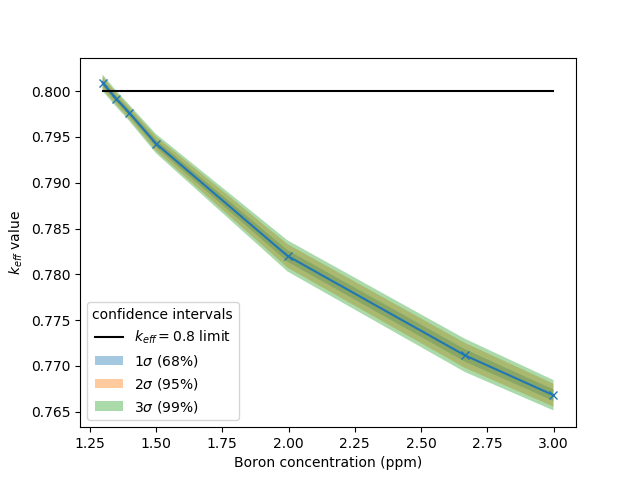
\includegraphics[height=5cm]{ConfidenceInterval.png}
\caption{The $\text{k}_{\text{eff}}$ only remains below 0.8 at boron concentration $\approx$ $<14$ ppm.
}\label{ConfInt}
\end{figure}

\begin{appendices}

\section{Figures}
\begin{figure}[H]
\centering
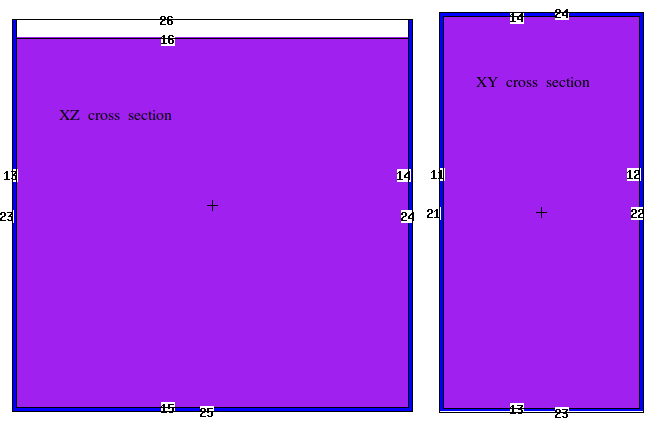
\includegraphics[height=6.4cm]{Ex1CrxSx.png}
\caption{The XZ and XY cross section of the bucket at the origin (z=0 and y=0 respectively)
}\label{Ex1CrxSx}
\end{figure}

\begin{figure}[H]
\centering
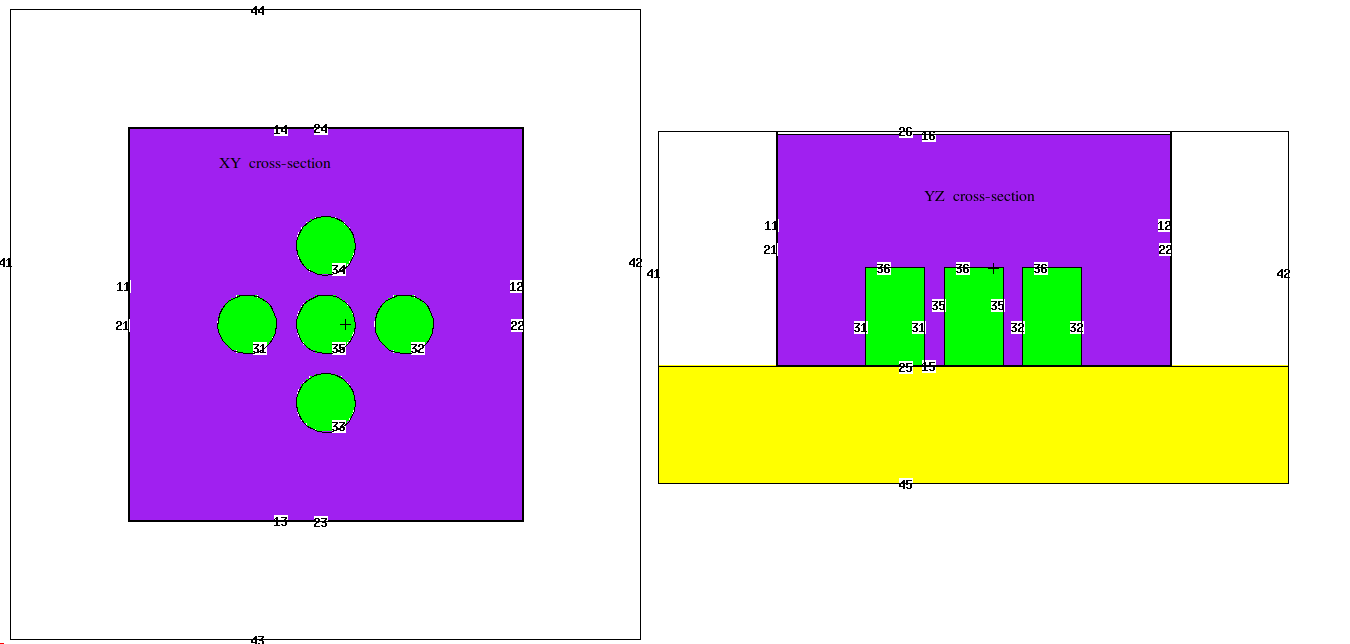
\includegraphics[height=6.4cm]{Ex3CrxSx.png}
\caption{The XY and YZ cross section of the bucket at the origin (z=0 and y=0 respectively)
}\label{Ex3CrxSx}
\end{figure}

\begin{figure}[H]
\centering
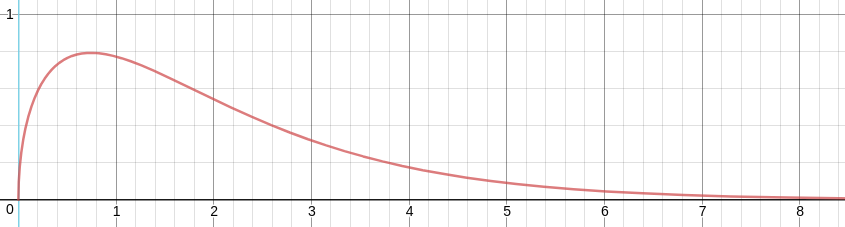
\includegraphics[height=3cm]{WattSpectrum.png}
\caption{Watt Spectrum (f=-3) using the parameters a=0.988,b=2.249 for fission of ${}^{235}$U by thermal neutron;
note the diminishing but non-zero probability of emission of high energy particles.
The x y axes has units of MeV and MeV$^{-1}$ respectively
}\label{Watt}
\end{figure}

\section{Tables}

\begin{table}[H]
\centering
\begin{tabular}{cc}
	${}^{1}_{1}$H  & 0.111894 \\
	${}^{16}_{8}$O & 0.888106
\end{tabular}
\caption{Isotopic compositions of pure water by weight fraction; density $\rho$=1.00g/cc, as given by [4]}\label{MaterialDef}
\end{table}
Need to insert table of
\\* materials
\\* (geometries?)
\section{References}
\indent

[1] MCNP4C2: Monte Carlo N-Particle Transport Code System Abstract (Diagnostics Applications Group, Los Alamos National Laboratory, Los Alamos, New Mexico.) p.2-160 (June 2001.)

[2] MCNP4C2: Monte Carlo N-Particle Transport Code System Abstract (Diagnostics Applications Group, Los Alamos National Laboratory, Los Alamos, New Mexico.) p.4-30 (June 2001.)

[3] MCNP4C2: Monte Carlo N-Particle Transport Code System Abstract (Diagnostics Applications Group, Los Alamos National Laboratory, Los Alamos, New Mexico.) p.2-180 (June 2001.)

[4] Compendium of Material Composition Data for Radiation Transport Modeling (R.G. Williams III, C.J. Gesh, R.T. Pagh) p.111 (April 2006)

\end{appendices}

\end{document}